\documentclass[12pt, a4paper]{article}
\usepackage[utf8]{inputenc}
\usepackage[T1]{fontenc}
\usepackage[english]{babel}
\usepackage{amsmath}
\usepackage{graphicx}
\usepackage{geometry}
\geometry{margin=2.5cm}
\usepackage[backend=biber,style=ieee,maxbibnames=99]{biblatex}
\addbibresource{references.bib}
\usepackage{hyperref}
\hypersetup{colorlinks=true, linkcolor=blue, citecolor=blue, urlcolor=blue}

\title{Mapping News Deserts in Denmark:\\ A Geospatial Analysis of Local News Coverage Across Municipalities}
\author{}
\date{}

\begin{document}
\maketitle

\noindent\textbf{Code availability.} All code and (most) data used to produce the results in this report are available at \url{https://github.com/Marieskau-hub/news-deserts-denmark}. The 114\,MB \texttt{kommuner.geojson} polygon file is hosted separately at Dataforsyningen (\url{https://dataforsyningen.dk/data/3901}).

\section{Introduction}
The decline of local journalism has emerged as a structural challenge to democratic governance, with research linking reduced local news presence to lower civic participation, increased political polarisation, and weakened institutional accountability \parencite{hayes2015, darr2018, adsera2003}. While this phenomenon has been extensively documented in the United States---particularly through the concept of ``news deserts'' \parencite{abernathy2020}---its applicability beyond the American context remains underexplored.

Denmark represents a critical case in this regard. Despite the historically resilient Nordic media model, characterised by high newspaper readership, strong public service broadcasting, and media subsidies designed to sustain pluralism \parencite{hallin2004, brink2009}, recent years have seen contractions in local news provision. Newsroom closures, declining advertising revenues, and increasing media concentration indicate a structural shift in the media landscape \parencite{cmpf2024denmark, reuters2024denmark}. Although policymakers have responded---most notably through the 2022--2025 Media Agreement---there remains no systematic, municipality-level understanding of how local news coverage is distributed across Denmark.

This paper addresses that gap by proposing a data-driven, spatially explicit approach to measuring variation in local journalism across Danish municipalities. The analysis combines a manually constructed newspaper-municipality dataset with population data and three socioeconomic covariates from Danmark Statistik: mean disposable income, the share of residents with a higher-education attainment, and voter turnout at the most recent published municipal election.

\section{Problems and Background}
Existing literature establishes the democratic importance of local journalism. Studies show that declining local news coverage is associated with lower voter turnout, increased political polarisation, and higher levels of corruption \parencite{hayes2015, darr2018, adsera2003}. However, the dominant conceptualisation of ``news deserts'' has largely been binary, classifying communities as either covered or not. As noted by \textcite{gulyas2023}, this obscures significant variation in coverage intensity across different areas.

In Denmark, research on the issue remains limited. The most substantial contribution to date, \emph{Det Sander Til} \parencite{oesterby2021}, identifies early signs of declining local coverage but does not provide systematic, spatially detailed mapping. Institutional analyses further suggest that news deserts are becoming a concern in Denmark, yet empirical evidence remains fragmented \parencite{cmpf2024denmark}.

This project is motivated by three interrelated problems. First, there is a lack of systematic, municipality-level data on local news coverage in Denmark. Second, existing approaches oversimplify the concept of news deserts by treating coverage as a binary condition rather than a matter of degree. Third, this lack of granular data creates policy blind spots, limiting the ability to target media subsidies and interventions effectively.

To address these challenges, digital tools play a central role. The project constructs a dataset by mapping local newspapers to municipalities using publicly available sources, and links this information to population data. Geospatial analysis techniques are used to visualise coverage patterns, while statistical methods---including spatial autocorrelation (Moran's~$I$) and correlation analysis---are applied to examine clustering and relationships with socioeconomic variables.

The approach follows three main steps. First, a dataset is manually constructed linking newspapers to municipalities. Second, a per-capita news coverage score is developed to capture coverage intensity as a continuous variable. Third, this measure is analysed through spatial visualisation, clustering analysis, and correlation with indicators such as income, education, and voter turnout.

Taken together, this provides both a methodological contribution---a replicable framework for mapping local news coverage in data-sparse contexts---and a substantive contribution by offering the first spatially explicit analysis of variation in local journalism across Danish municipalities.

\section{Data acquisition and processing}
\subsection{Data Sources}
The primary data source for identifying local newspapers and their coverage area is MediaVejviseren, which provides directory-level information on Danish media outlets. This is supplemented by data from the Danish Ministry of Culture, which includes information on media support and registered publications. Together, these sources are used to identify local weekly newspapers and assign them to the municipalities they serve.

Population data is obtained from Danmarks Statistik, providing municipality-level figures used to normalise coverage measures. In addition, socioeconomic indicators---including average income, educational attainment, and voter turnout---are collected from official statistical sources to enable subsequent correlation analysis.

\subsection{Data Construction}
The dataset is constructed through a manual mapping process in which each identified local newspaper is assigned to one or more municipalities based on its stated coverage area. This process involves interpreting descriptive information from directories and, where necessary, consulting newspaper websites to clarify geographic scope.

The unit of analysis is the municipality. For each municipality, the total number of local newspapers covering the area is recorded. Because newspapers may cover multiple municipalities, the mapping allows for one-to-many relationships between newspapers and municipalities.

This resulted in a structured dataset in which each municipality is associated with
\begin{itemize}
    \item The number of local newspapers covering the area
    \item Population size
    \item Socioeconomic indicators (income, education, voter turnout)
\end{itemize}

\subsection{Processing and Feature Construction}
To move beyond a binary understanding of news presence, a per-capita news coverage score is constructed. This metric captures the density of local journalism relative to population size and is defined as
\[
\text{Coverage Score}_i = \frac{\text{Number of Newspapers}_i}{\text{Population}_i}
\]
where $i$ denotes the municipality.
This transformation enables comparison across municipalities of different sizes and provides a continuous measure of coverage intensity. The resulting variable serves as the primary dependent variable in the analysis.

Data processing is conducted using Python, where datasets are cleaned, merged and transformed. Some of the steps include:
\begin{itemize}
    \item Standardising municipality names across datasets to ensure consistent joins
    \item Handling missing values in socioeconomic indicators
    \item Normalising variables where necessary for comparability
\end{itemize}

\subsection{Analytical preparation}
The processed dataset was then prepared for three types of analysis. First, geospatial data structures are created to enable choropleth mapping of coverage scores across municipalities. Second, spatial weights matrices are constructed to support spatial autocorrelation analysis (Moran's~$I$), allowing for the identification of geographic clustering in low- or high-coverage areas. Third, the dataset is structured for statistical analysis, enabling correlation tests between coverage scores and socioeconomic variables.

Given the manual nature of the data construction process, the dataset should be understood as a proof-of-concept. While care is taken to ensure accuracy, the mapping of newspapers to municipalities is dependent on publicly available descriptions and may not fully capture variations in actual editorial coverage.

\section{Results}
\subsection{Coding template}
The completed coding template contains 60 newspaper-to-municipality mapping rows. These rows describe 34 unique newspapers covering 22 unique municipalities within Region Syddanmark. Two structural features of the dataset are worth noting before the spatial results.

First, the publisher landscape is highly concentrated. Jysk Fynske Medier (JFM) publishes 31 of the 34 unique newspaper titles in the dataset (91.2\%) and accounts for 51 of the 60 newspaper-municipality mapping rows (85.0\%). JFM's titles are distributed across regional dailies (\emph{JydskeVestkysten} and \emph{Fyens Stiftstidende}) and a network of weekly free-distribution titles (Ugeavisen-branded papers and equivalents). The remaining 9 mapping rows (15.0\%) correspond to three non-JFM titles: \emph{Der Nordschleswiger}, the German-minority daily published by BDN/Deutscher Presseverein and covering Haderslev, Sønderborg, Aabenraa and Tønder (4~rows); \emph{Sydnyt.dk}, an independent digital outlet covering the same four Sønderjylland municipalities (4~rows); and \emph{AVISEN for Gråsten, Lundtoft og Sundeved}, a single weekly free-distribution paper of unknown publisher in Sønderborg (1~row).

Second, regional dailies create one-to-many mapping rows. \emph{JydskeVestkysten} and \emph{Fyens Stiftstidende} each cover exactly ten municipalities individually, which means that a single newspaper title is counted once per municipality it serves. This is a deliberate methodological choice: from a reader's perspective, the relevant question is whether at least one newspaper covers their municipality, not how many municipalities the newspaper as an organisation covers in total.

\subsection{Per-capita coverage score}
For each municipality, the per-capita coverage score is computed as the number of
newspapers covering that municipality divided by population, expressed per 10{,}000
residents:
\begin{equation*}
    \text{score\_per\_10k} = \frac{\text{newspaper\_count}}{\text{population}} \times 10{,}000
\end{equation*}
Across the 23 study-area municipalities, the mean score is 0.621 papers per 10{,}000
residents and the median is 0.573. The full distribution ranges from 0.000 (Fanø,
the only municipality in the study area with no mapped newspaper) to 1.734 (Ærø).
The five highest-scoring municipalities are all small in population:
\begin{itemize}
    \item Ærø --- 1.734 per 10k (population 5{,}766; one paid daily edition)
    \item Langeland --- 1.689 per 10k (population 11{,}841; two papers)
    \item Tønder --- 1.106 per 10k (population 36{,}174; four papers)
    \item Kerteminde --- 0.823 per 10k (population 24{,}299; two papers)
    \item Fredericia --- 0.756 per 10k (population 52{,}939; four papers)
\end{itemize}
At the opposite end, the lowest non-zero scores belong to the most populous municipalities in the study area: Odense at 0.094 per 10k (population 213{,}168, two papers), Horsens at 0.202 per 10k (population 98{,}806, two papers), Kolding at 0.312 per 10k (population 96{,}214, three papers), and Vejle at 0.325 per 10k (population 123{,}250, four papers). This inverse relationship between population size and per-capita score is examined quantitatively at the end of this section and discussed in Section~\ref{sec:bias}.
\begin{figure}[h]
    \centering
    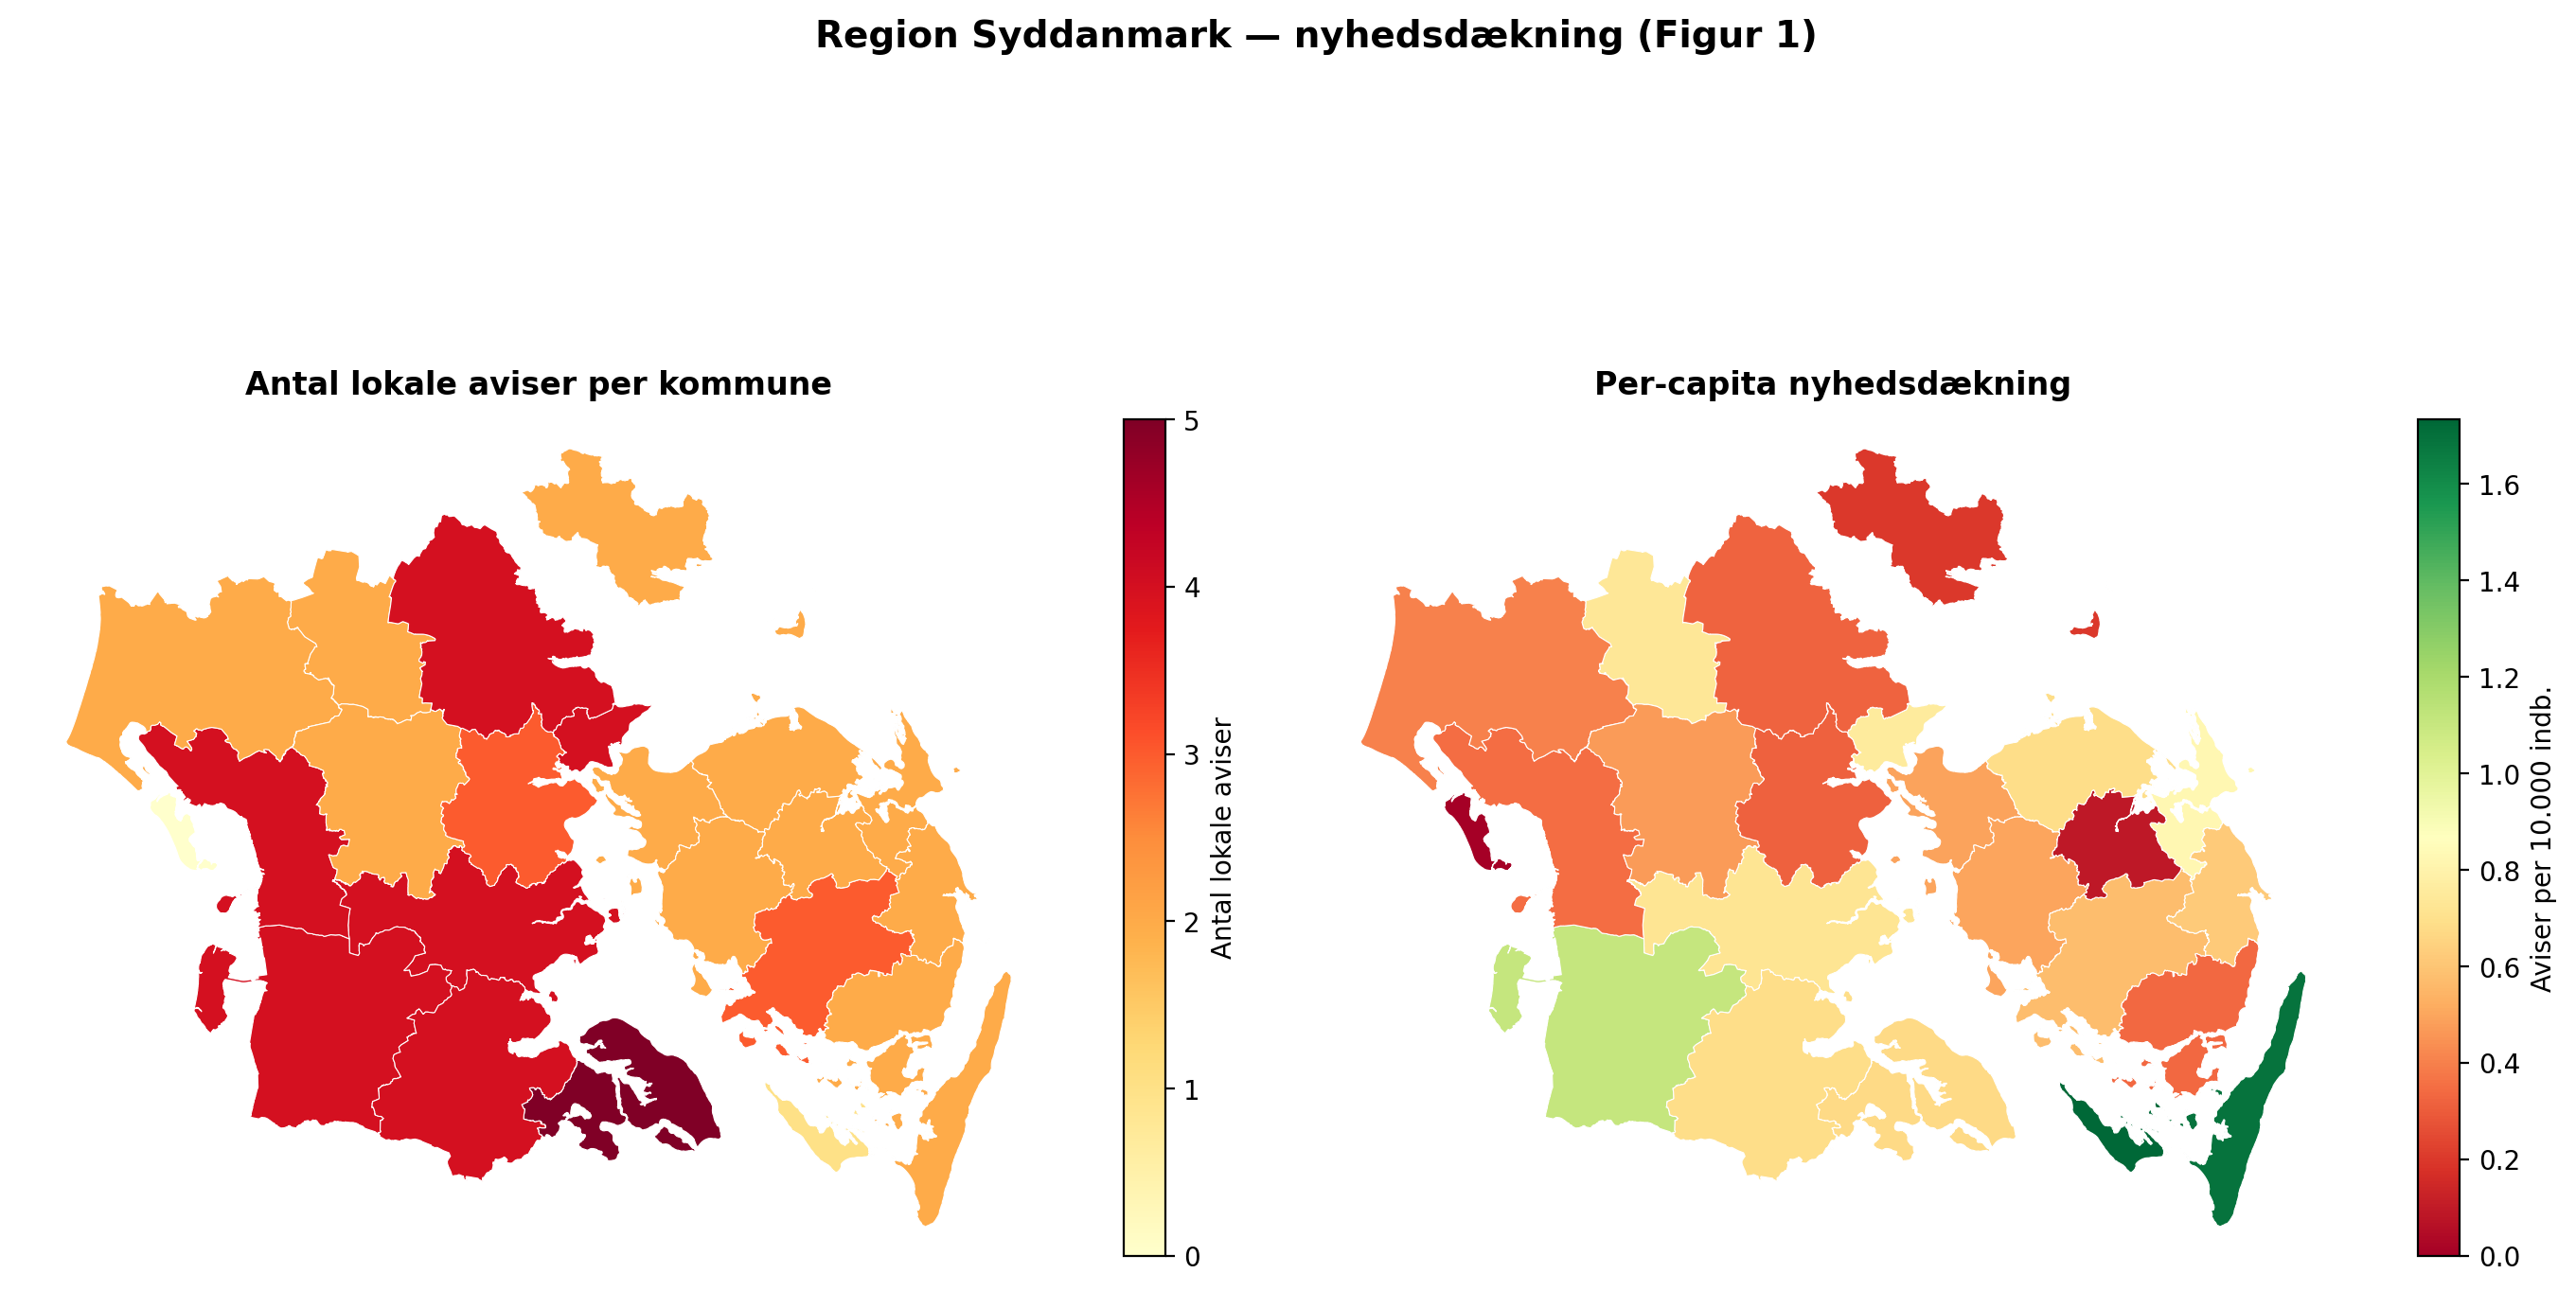
\includegraphics[width=0.85\textwidth]{choropleth_syddanmark.png}
    \caption{Per-capita news-coverage score (papers per 10{,}000 residents) for the
    23-municipality study area. Darker shading indicates higher coverage relative
    to population.}
    \label{fig:choro}
\end{figure}
\begin{figure}[h]
    \centering
    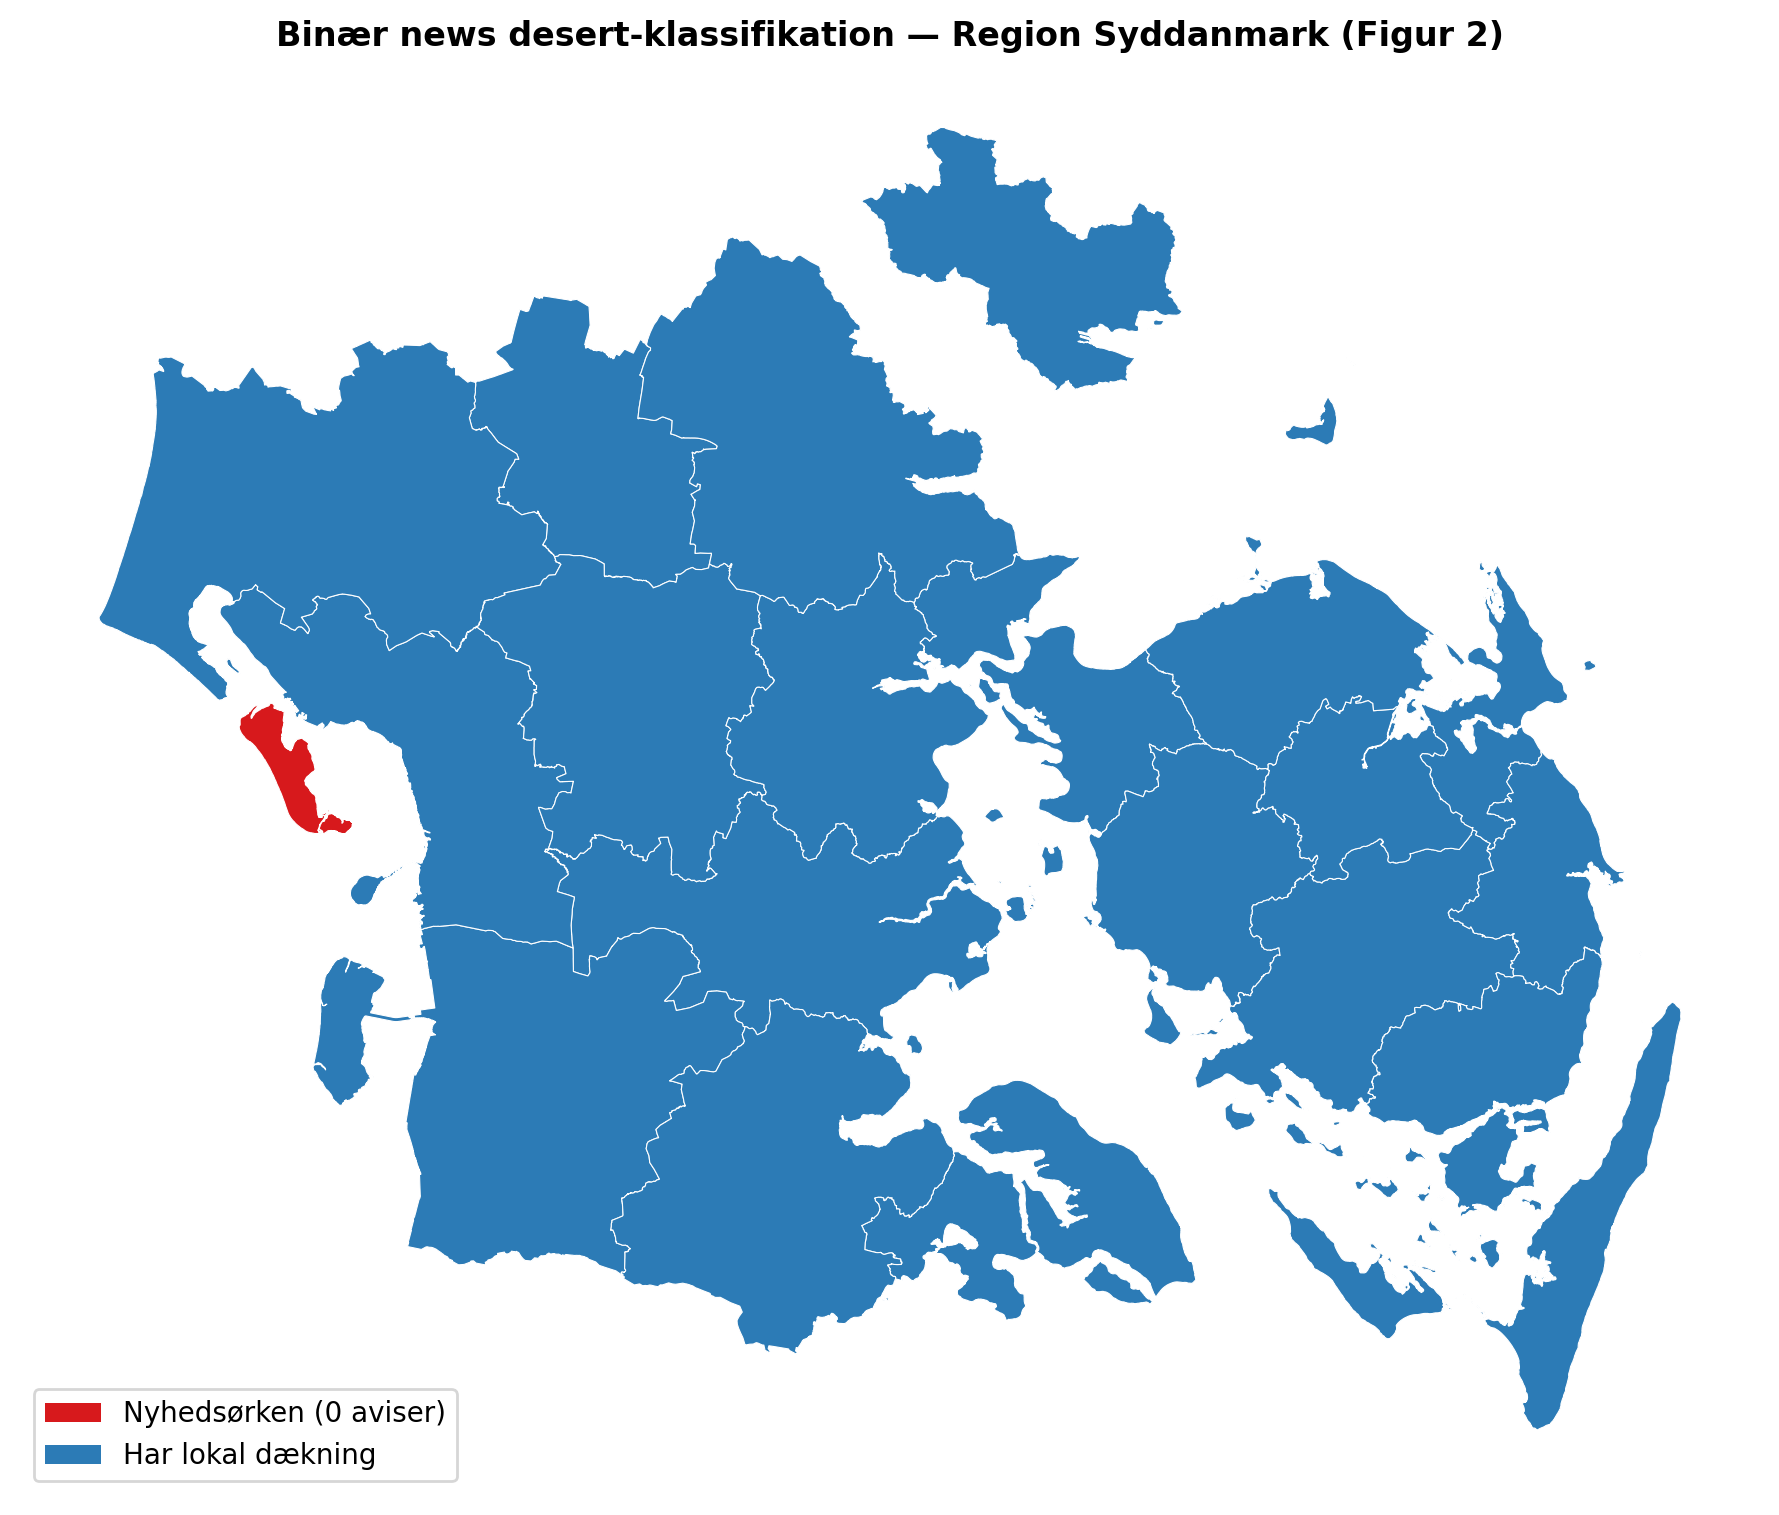
\includegraphics[width=0.85\textwidth]{news_deserts_binary_syd.png}
    \caption{Binary news-desert classification: a municipality is flagged as a news
    desert when newspaper\_count = 0. Within the study area only Fanø meets this
    definition.}
    \label{fig:binary}
\end{figure}
Under a strict definition (newspaper\_count = 0), Fanø is the only news desert in
the study area. Its population of 3{,}332 is served by no newspaper that appears in the coding template --- \emph{JydskeVestkysten}'s coverage of the Esbjerg area does
not include a Fanø-specific edition or section in the mapping. All other 22
municipalities have at least one mapped newspaper.

\subsection{Spatial autocorrelation: Global and Local Moran's~$I$}
Spatial autocorrelation tests whether municipalities with similar per-capita scores tend to cluster geographically. Two spatial-weight specifications were used to ensure the result is not driven by the choice of neighbourhood:
\begin{itemize}
    \item \textbf{Queen contiguity weights} --- municipalities sharing a border or
    a vertex are neighbours. Under this specification four units in the study area
    are islands with no land neighbours (Langeland, Ærø, Fanø, and the
    inland-disconnected Horsens-as-Syddanmark assignment), generating a warning
    about disconnected components.
    \item \textbf{$k$-nearest-neighbours (KNN, $k = 4$) weights} --- every
    municipality has exactly four neighbours, eliminating the island problem at the
    cost of imposing equal connectivity on all units.
\end{itemize}
Under the Queen specification, Global Moran's $I = -0.012$ with $p = 0.394$ (999
permutations). Under the KNN-4 specification, Global Moran's $I = 0.098$ with
$p = 0.123$. Neither specification rejects the null hypothesis of spatial
randomness at the conventional $\alpha = 0.05$ threshold. In substantive terms,
this means that --- in this study area, with this score, and with these 23 units --- there is no statistically detectable global tendency for high-coverage or low-coverage municipalities to cluster.
\begin{figure}[h]
    \centering
    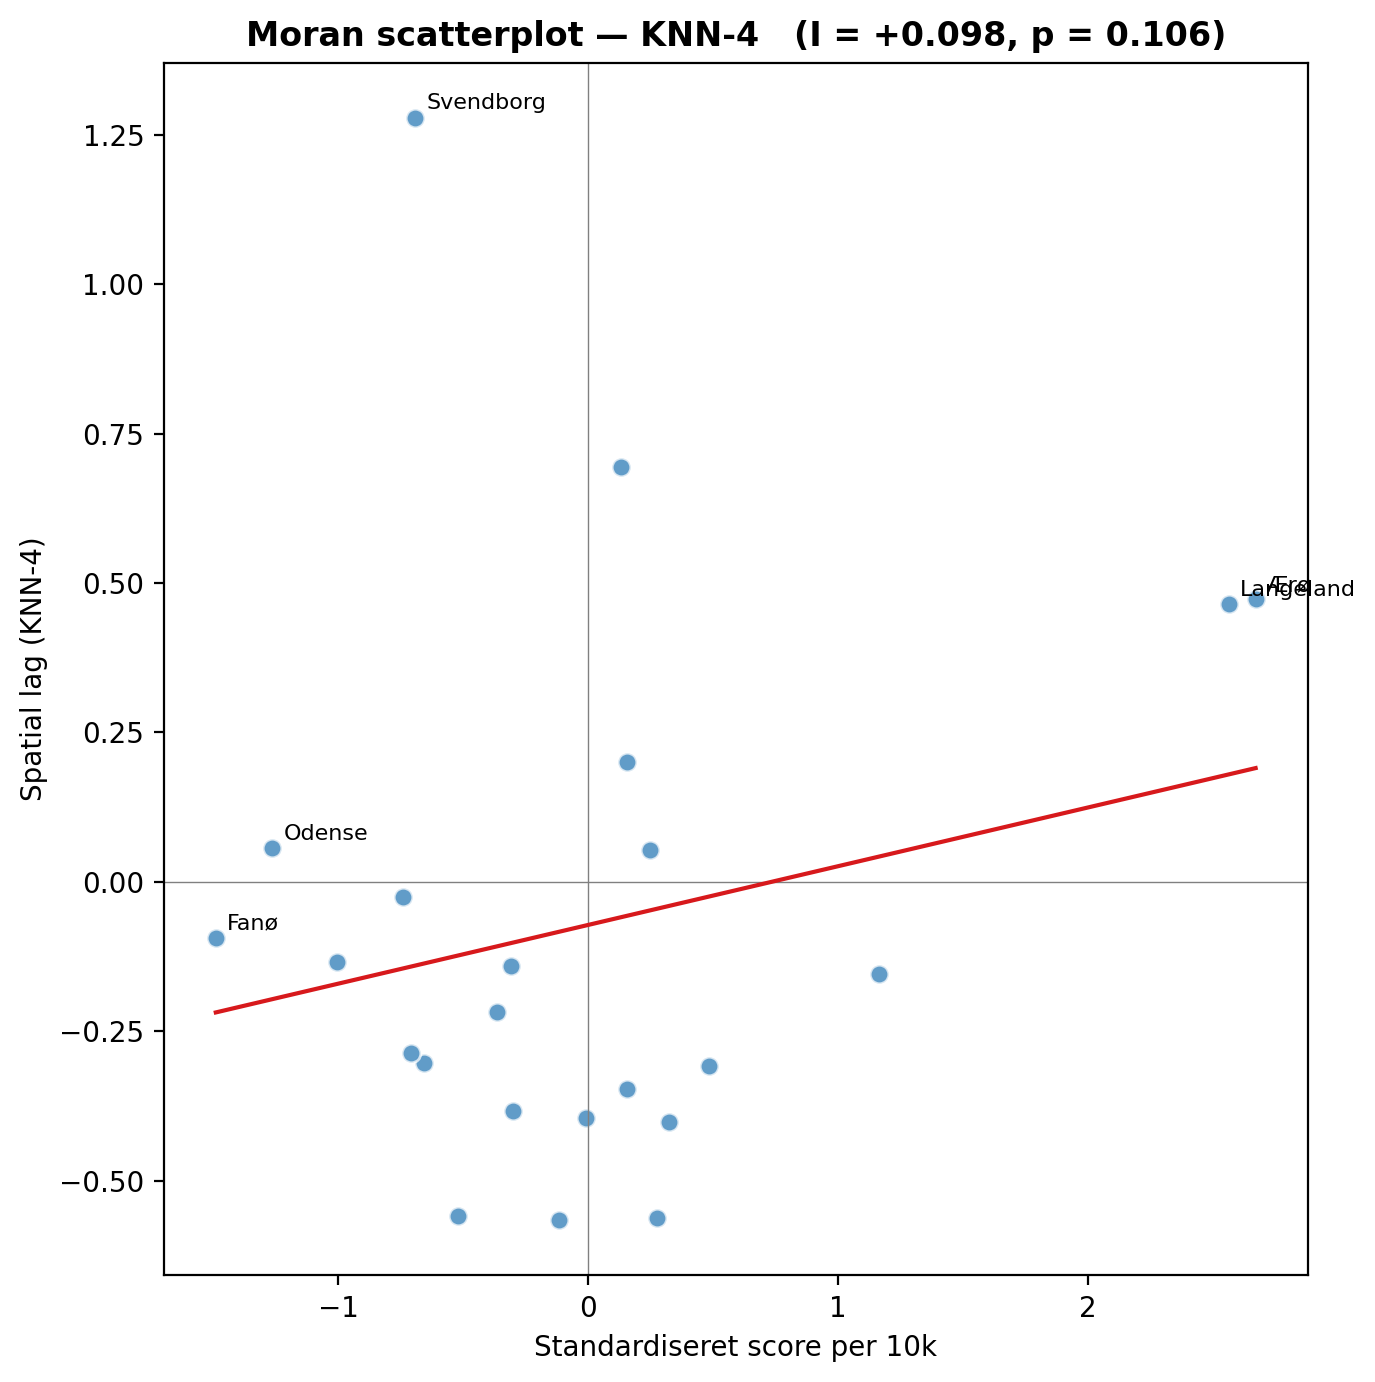
\includegraphics[width=0.7\textwidth]{moran_scatter_syd.png}
    \caption{Moran scatterplot of standardised per-capita score vs.\
    spatially-lagged standardised score (KNN-4 weights). The slope (Moran's~$I$) is
    $0.098$ and is not statistically significant at $\alpha = 0.05$.}
    \label{fig:moran}
\end{figure}
Local Moran's $I$ (LISA) was computed with the same KNN-4 weights to look for
individual outlier municipalities even where the global statistic is not
significant. Of the 23 units, exactly one is significant at $p < 0.05$: Svendborg
(LISA $p = 0.007$), classified as a Low-High outlier --- i.e.\ a comparatively
low-scoring municipality (0.333 per 10k) surrounded by higher-scoring neighbours on
Funen. No High-High or Low-Low cluster was detected at the 0.05 level. Several
municipalities (Sønderborg, Faaborg-Midtfyn, Varde, Ærø, Langeland, Billund)
approach significance ($0.05 \le p < 0.11$) but do not cross the conventional
threshold.
\begin{figure}[h]
    \centering
    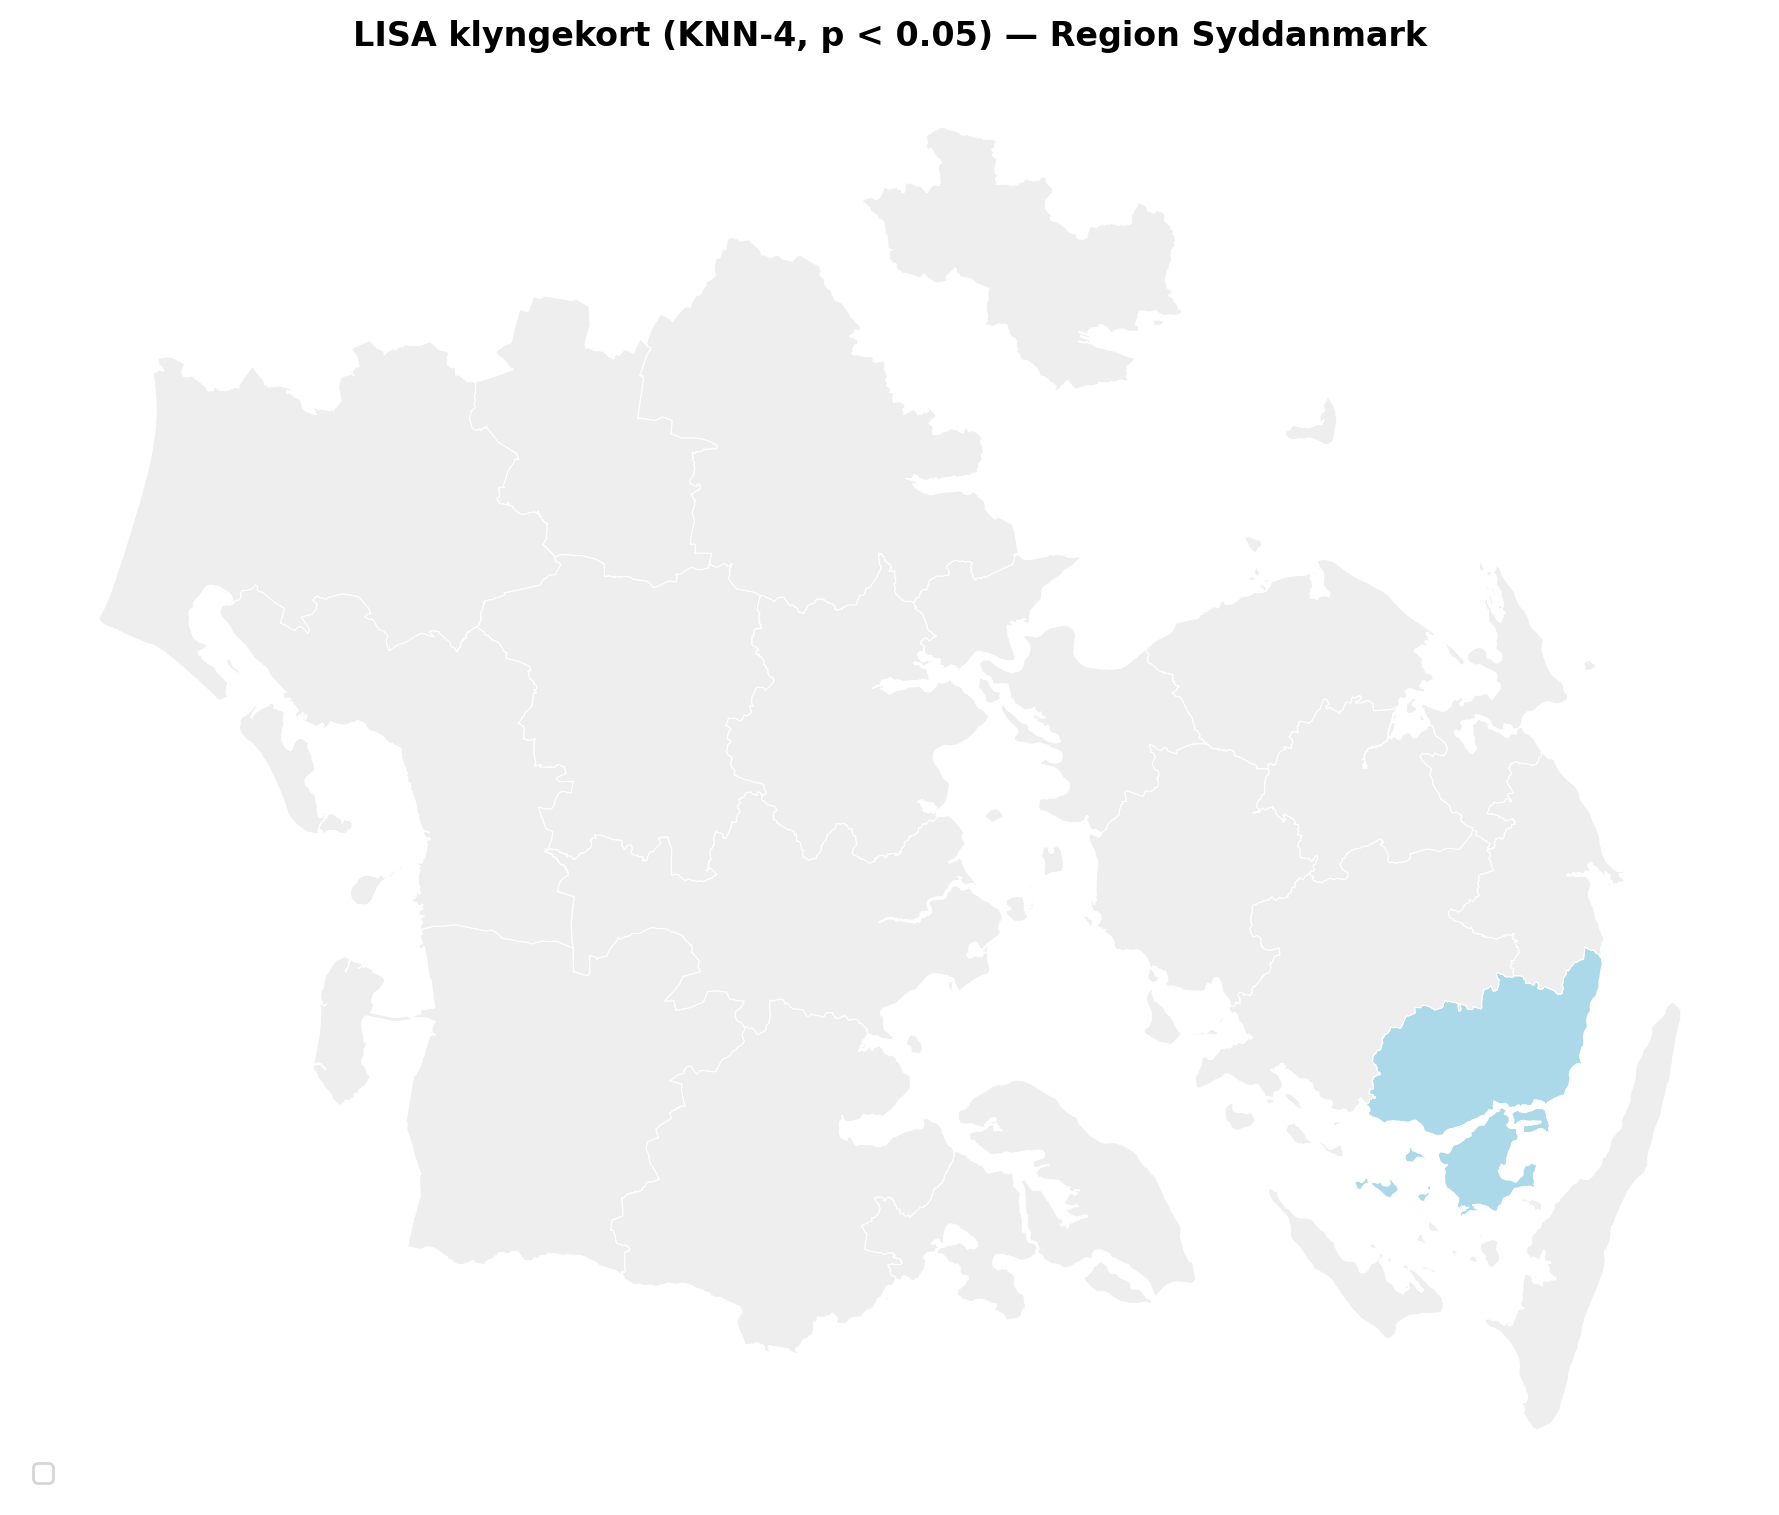
\includegraphics[width=0.85\textwidth]{lisa_clusters_syd.png}
    \caption{Local Moran's~$I$ (LISA) cluster map (KNN-4 weights, $p < 0.05$). Only
    Svendborg is significant, classified as a Low-High outlier.}
    \label{fig:lisa}
\end{figure}

\subsection{Coverage and population size}
\label{sec:popcorr}
Although Moran's~$I$ does not detect spatial clustering, a different --- and
methodologically important --- pattern is visible in the data: per-capita coverage
is strongly negatively correlated with population. The Spearman rank correlation
between population and \texttt{score\_per\_10k} across the 23 study-area
municipalities is $\rho = -0.558$ with $p = 0.006$. Visually, this is the same
effect that produces the contrast in Figure~\ref{fig:choro} between the small
islands and Fyn-rural municipalities (high per-capita scores) and the large urban
centres of Odense, Horsens, Kolding, and Vejle (low per-capita scores).
This is partly an arithmetic artefact of the score's denominator: a regional daily
that covers Odense counts as one paper for 213{,}168 residents, while the same
daily counted for Ærø covers 5{,}766 residents. It is also partly a coding
artefact: the template captures editions and titles, not editorial intensity per
municipality. A regional daily's Odense bureau likely produces far more
Odense-relevant journalism per capita than its Ærø bureau, but this dimension is
not in the coding scheme. The implication for interpretation is discussed in
Section~\ref{sec:bias}.

\subsection{Socioeconomic Correlations}
To explore whether variation in news coverage aligns with broader municipal
differences, the coverage score is compared with three socioeconomic indicators
drawn from Statistics Denmark's Statbank: mean disposable income per person (table
INDKP101, 2024, all persons, INDKOMSTTYPE~$=100$, ENHED~$=116$), the share of
residents aged 15--69 with a higher-education attainment at the bachelor (H60) or
long higher-education (H70) level (HFUDD10, 2019), and voter turnout at the most
recent published municipal election (KVRES, KV21 --- November 2021; the November
2025 election results were not yet available in Statbank at the time of analysis).
This part of the analysis is exploratory. The aim is not to establish a causal
relationship between local news coverage and socioeconomic conditions, but rather
to examine whether municipalities with weaker relative coverage also display other
forms of civic or economic disadvantage.
For each variable, Spearman rank correlation with the per-capita coverage score
(\texttt{score\_per\_10k}) was computed across the 23 study-area municipalities.
Spearman was preferred over Pearson because the per-capita score is right-skewed by
the small-population units (Ærø, Langeland) and rank correlation is robust to that
skew.
\begin{table}[h]
\centering
\caption{Spearman rank correlations of per-capita coverage score with three
socioeconomic variables, 23-municipality study area. Pearson $r$ reported alongside
for reference.}
\label{tab:correlations}
\begin{tabular}{lrrrrr}
\toprule
\textbf{Socioeconomic variable} & \textbf{Spearman~$\rho$} & \textbf{$p$}
                                & \textbf{Pearson~$r$} & \textbf{$p$}
                                & \textbf{$n$} \\
\midrule
Mean disposable income (kr.) & $-0.577$ & 0.004 & $-0.478$ & 0.021 & 23 \\
Higher-education share (\%)  & $-0.630$ & 0.001 & $-0.572$ & 0.004 & 23 \\
Voter turnout, KV21 (\%)     & $+0.265$ & 0.222 & $+0.270$ & 0.212 & 23 \\
\bottomrule
\end{tabular}
\end{table}
Two of the three associations are statistically significant at $\alpha = 0.05$ and
both are negative: per-capita coverage decreases as mean income rises (Spearman
$\rho = -0.577$, $p = 0.004$) and as the higher-education share rises (Spearman
$\rho = -0.630$, $p = 0.001$). Voter turnout shows a positive but non-significant
association (Spearman $\rho = +0.265$, $p = 0.222$).
The two significant negative associations are most plausibly read as a downstream
consequence of the per-capita score's bias toward small, low-population
municipalities, rather
than as evidence that affluent or well-educated residents are systematically
under-served by local newspapers. The largest, most affluent, and best-educated
municipalities in the study area --- Odense, Vejle, Kolding, and Horsens --- are
also the ones whose per-capita scores are mechanically depressed by their large
population denominators. The non-significant positive turnout association points in
the direction the news-deserts literature would predict (more local coverage
$\rightarrow$ more civic engagement) but does not survive a conventional
significance threshold at this $N$. A robustness check that excludes Horsens
($N = 22$, the official Region Syddanmark municipality count) leaves all three
correlations qualitatively unchanged: $\rho = -0.574$ ($p = 0.005$) for income,
$\rho = -0.601$ ($p = 0.003$) for education, and $\rho = +0.188$ ($p = 0.402$) for
turnout.

\section{Critical evaluation}
\subsection{Per-capita score is biased toward small municipalities}
\label{sec:bias}
Population-normalising newspaper counts produces a strong mechanical correlation between population and score (Spearman $\rho = -0.558$, $p = 0.006$;
Section~\ref{sec:popcorr}). Odense's 0.094 versus Kerteminde's 0.823 reflects denominators, not editorial intensity: the same regional daily is divided across very different population bases.

\subsection{Horsens is in Region Midtjylland, not Syddanmark}
\texttt{dk\_municipalities.csv} labels Horsens (kommune-kode 615) as Syddanmark,
but it administratively belongs to Region Midtjylland. It is retained here because
the JFM coverage area extends into Horsens; the ``Region Syddanmark'' results
should therefore be read as ``the JFM footprint in and adjacent to Syddanmark''.

\subsection{Publisher concentration is a structural risk}
JFM publishes 91.2\% of unique titles and accounts for 85.0\% of mapping rows. The
score measures presence, not pluralism: two JFM titles in one municipality look
identical to one JFM and one independent. An effective-number-of-publishers index
would surface this dimension and capture the latent risk that any editorial
consolidation by JFM would create news deserts simultaneously across many
municipalities.

\subsection{Manual coding limitations}
Coverage is binary at the municipality level; edge cases (weekend-only sections, partial-distribution weeklies) are simplified. The dataset is a 2026 cross-section so no longitudinal claims are made.

\subsection{Non-significant Moran's~$I$ is itself a result}
Both specifications (Queen $p = 0.394$; KNN-4 $p = 0.123$) fail to reject spatial
randomness. With only $N = 23$ units, a population-tied score, and regional dailies
that span many adjacent municipalities by construction, this is unsurprising. The
sole LISA outlier is Svendborg (Low-High). A national-scale rerun ($N \approx 98$)
would have substantially more power.

\subsection{Caveats on the socioeconomic variables}
The income measure is \emph{mean} disposable income (INDKP101,
INDKOMSTTYPE~$=100$, ENHED~$=116$, 2024); mean and median are highly
rank-correlated across Danish municipalities, but a strict-median rerun is
recommended. Voter turnout is KV21, because KV25 results were not yet in Statbank
at the time of analysis (April 2026); the column should be re-pulled and the
correlations re-run once published.

\subsection{Choice of spatial weights}
Queen contiguity produces disconnected components (Langeland, Ærø, Fanø, and the
Horsens assignment have no land neighbours in the study area), so KNN-4 was used
as a robustness check. Both specifications give the same qualitative answer, so
the conclusions are not driven by the weighting choice.

\section{Conclusions and future work}
Three conclusions follow from the analysis:
\begin{itemize}
    \item News-desert prevalence under a strict (\texttt{newspaper\_count} = 0) definition is low in the study area: only Fanø (population 3{,}332) qualifies. The methodological pipeline is, however, fully operational and can be re-run on any region or on Denmark as a whole.
    \item Per-capita coverage is dominated by population size rather than by geography. The Spearman correlation between population and \texttt{score\_per\_10k} is $-0.558$ ($p = 0.006$), and Global Moran's $I$ is non-significant under both Queen and KNN-4 weights. There is no statistical evidence of regional clusters of high or low coverage at this scale.
    \item The publisher-concentration finding is itself a result. With JFM
    publishing 31 of 34 unique titles (91.2\%) and accounting for 85.0\% of the
    mapping rows, the news-desert risk in the study area is best understood as a
    structural exposure to a single publisher's editorial decisions, not as a
    geographic clustering pattern.
 \end{itemize}
\printbibliography

\end{document}
